% Clean AI-assisted research revision, 20 October 2026.
% The preserved supervisor source is paper_history/supervisor_draft.tex.
% Author metadata and declarations need human approval before submission.
\documentclass[5p,times,twocolumn]{elsarticle}
\usepackage[T1]{fontenc}
\input{glyphtounicode}
\pdfgentounicode=1
\usepackage{graphicx,multirow}
\usepackage{amsmath,amssymb,amsfonts,amsthm}
\usepackage{xcolor,textcomp,booktabs,tabularx,array,adjustbox}
\usepackage{placeins,dblfloatfix,listings,enumitem,url}
\usepackage{needspace}
\usepackage[hidelinks]{hyperref}
\setlength{\emergencystretch}{2em}
\Urlmuskip=0mu plus 1mu
\newcolumntype{Y}{>{\raggedright\arraybackslash\hspace{0pt}}X}
\newcolumntype{R}{>{\raggedleft\arraybackslash\hspace{0pt}}X}
\newcolumntype{C}{>{\centering\arraybackslash\hspace{0pt}}X}
\newcommand{\newtext}[1]{#1}
\theoremstyle{plain}
\newtheorem{theorem}{Theorem}
\newtheorem{proposition}[theorem]{Proposition}
\newtheorem{corollary}[theorem]{Corollary}
\newtheorem{lemma}[theorem]{Lemma}
\theoremstyle{definition}
\newtheorem{definition}{Definition}
\theoremstyle{remark}
\newtheorem{remark}{Remark}
\raggedbottom
\setlength{\tabcolsep}{3pt}
\setlength{\dblfloatsep}{12pt plus 2pt minus 2pt}
\setlength{\dbltextfloatsep}{14pt plus 2pt minus 2pt}
\renewcommand{\dblfloatpagefraction}{0.65}
\journal{Neurocomputing}

\begin{document}
\begin{frontmatter}
\title{Verifiable Center-Based Clustering with Reusable Statistics and Integer Accuracy Certificates}
\author{Author information pending confirmation}
\begin{abstract}
Auditing nearest-center assignments over private high-dimensional records is expensive when successive proofs repeat original-space distances. We implement a two-stage zero-knowledge system that binds compact head coordinates and residual energy to committed records and reuses them across public center updates. An optional integer certificate proves a lower bound on the number of correct original-space assignments and an interval containing the exact quantized nearest-center cost, accounting for the Gram defect of the rounded basis. A public-only verifier checks approved centers, subsets and proof coverage before an explicit accuracy policy is applied. We evaluate exact public-center Full, equally reusable PCA/energy and plain and certified learned reuse on one four-CPU host. All 14 controls finish, including actual 1,024-record audits over ten center sets; 6,848 proofs pass independent public-only replay. At this scale, measured component costs are 24,681.3 seconds for exact Full, 4,778.1 for plain learned reuse and 4,861.0 for certified reuse. Certification adds 1.74\% to total cost. Across nine updated sets, observed quantized assignment agreement is 98.25\%, but certified coverage averages 61.63\% and cost-interval width 20.65\%. A completed higher-rank 256-record configuration improves agreement to 99.74\% and certified coverage to 85.20\%, with increased total cost. No updated set meets a strict 99\% coverage / 1\% width policy. The contribution is an authenticated reusable audit interface with checked integer approximation guarantees and a measured computation--accuracy trade-off; the lower costs do not establish equal-fidelity acceleration of exact computation.
\end{abstract}
\begin{keyword}
zero-knowledge proofs \sep verifiable clustering \sep reusable statistics \sep dimensionality reduction \sep privacy-preserving computation
\end{keyword}
\end{frontmatter}

\section{Introduction}\label{sec:introduction}
A data owner may need to demonstrate that public cluster centers give a reported assignment cost on private records. Examples include an analyst checking a deployed model on sensitive embeddings and an auditor requesting costs for several proposed model updates. Zero-knowledge proofs establish the specified computation without disclosing its private witness \cite{gmr1991knowledge,groth2016}. The difficulty is repeated high-dimensional arithmetic: a direct nearest-center audit evaluates distances in $d$ dimensions for every record and every candidate center. In the completed 1,024-record MNIST control, our exact public-center Groth16 circuit requires 1.43 million constraints for a batch of eight 784-dimensional records.

The same committed records can be queried many times. This motivates a two-stage construction. Stage~1 proves once that compact statistics were derived correctly from every committed original row. Stage~2 authenticates the requested statistics and proves nearest-center assignments and their aggregate cost. The central systems question is which statistics allow useful later queries while avoiding repeated original-space work.

For one fixed center set, the geometry is elementary. An orthonormal basis spanning the center differences preserves all assignment comparisons; adding each record's squared residual norm recovers every center distance. This follows from Pythagoras and belongs to the established projection-plus-offset approach to clustering sketches \cite{feldman2013tiny,feldman2020tiny,cohen2015dimensionality}. We use this identity as an interface to a proof system. We do not propose a new dimensionality-reduction identity or a new coreset theorem.

Fixed-center answers alone are insufficient to justify a reusable representation. A stronger task-specific baseline computes and proves the exact winning center and minimum cost in Stage~1, then authenticates those two values in later subset queries. It is cheaper for a single fixed center set. Exact affine scores provide another compact baseline with the same fixed-center information. Both measured implementations specialize preprocessing to the selected centers, so their Stage~1 work is repeated when those centers change.

We therefore study audits under changing public centers. An analyst can compare proposed prototype updates against the same sensitive embedding catalog without disclosing individual records or assignments to an auditor. We augment the deployed-center span with principal components of training residuals, and store the resulting head coordinates and residual energy. New centers enter Stage~2 through public head coordinates and residual offsets. They change the query inputs without changing the catalog or the query setup. This yields an exact real-arithmetic distance when the new centers remain in the represented affine span, and an approximation otherwise. The approximation drops a residual cross term. Proving this approximate execution alone does not establish original-space accuracy. We add a circuit-checked error envelope that accounts for both the omitted cross term and the nonorthogonality of the rounded basis, yielding per-set cost intervals and certified assignment counts.

An exact method can also reuse setup: put the full centers in the public statement and compute original-space distances directly. We implement this public-center Full circuit and prove complete catalogs with it. The earlier 6.82--7.76-fold savings over center-specific caches are retained only as a historical implementation comparison. The completed serial campaign measures matched plain reuse, certified reuse and public-center Full, including an actual 1,024-record catalog and predeclared higher-rank controls. At 1,024 records, learned plain and certified reuse have 5.17- and 5.08-fold lower measured component cost than exact public-center Full. These alternatives provide different fidelity guarantees: the certificate can force an auditor to refuse an inexpensive approximate answer.

The contribution has three parts:
\begin{enumerate}[leftmargin=*]
\item An original-data-bound integer audit interface, with complete Stage~1 coverage, public-center reuse and independent public-only verification against approved tasks.
\item An optional rounded-basis accuracy relation: private row statistics yield a public lower bound on correct original-space assignments and an interval for exact quantized cost. An explicit policy can refuse a valid approximate proof when these bounds are insufficient.
\item A completed matched evaluation against exact public-center Full and equally reusable PCA/energy, including actual 1,024-record proofs, measured certificate overhead and higher-rank proof controls. All 6,848 campaign proofs pass public-only replay; historical timing cohorts and native budget grids remain separate.
\end{enumerate}

\section{Related work}\label{sec:related}
\paragraph{Projection and residual offsets}
Feldman, Schmidt and Sohler reduce clustering dimension while retaining an additive cost independent of the queried solution \cite{feldman2013tiny,feldman2020tiny}. Their arXiv extended version states the matrix Pythagorean identity (Claim~3) and, for centers in a subspace, the decomposition into projection cost and orthogonal residual cost (Eq.~9). Cohen et al. formalize projection-cost-preserving sketches with a solution-independent additive constant \cite{cohen2015dimensionality}. These results address approximation over classes of clustering solutions. Here we keep one energy value per authenticated record so that arbitrary requested subsets can be audited, and prove the deterministic derivation from the original commitment. The fixed-center identity is a special case of this classical geometry; the reuse circuit and its measured trade-offs are the focus.

\paragraph{Verifiable clustering and private analytics}
Prior work already combines private $k$-means and zero-knowledge techniques. Duan and Canny use random projections in zero-knowledge checks of vector norm bounds for private distributed data mining \cite{duan2008private}. Patel, Patel and Jinwala use secret sharing with a code-based identification scheme for horizontally partitioned clustering against malicious participants \cite{patel2013clustering}. Zhang, Li and Chang describe verifiable outsourced privacy-preserving $k$-means using secure distance and minimum computations \cite{zhang2021verifiable}. Repetto et al. prove PAC-private mechanisms, including $k$-means, using RISC-Zero \cite{repetto2026pac}. These works address input validity, distributed computation or outsourced clustering, whereas our task audits successive public center sets against an unchanged committed catalog. In nearby vector search, V3DB proves execution of published approximate-search semantics over committed snapshots \cite{v3db2026}. Our relation instead proves exhaustive nearest-center comparisons on authenticated statistics and checks an envelope for original-space quantized answers. Neither projection-based ZK checks, ZK clustering nor audits over committed vector data are new categories.

\paragraph{Proof-oriented representations}
ezDPS studies a ZK inference pipeline including PCA, and Artemis develops commit-and-prove techniques for external data or model commitments \cite{ezdps2023,artemis2024}. Our PCA baseline proves an approved projected computation in the same backend; it does not reproduce ezDPS or prove PCA training. We use Groth16 over BN254 and Poseidon2 row-Merkle authentication \cite{groth2016,poseidon22023}. The contribution is a representation and circuit design within this setting, not a new proof primitive.

\paragraph{Privacy-preserving prototype models}
Schubert et al. implement a nearest-prototype learning model using fully homomorphic encryption and study the effects of integer encoding and distance computation \cite{schubert2026prototype}. Their objective is computation over encrypted data. Our objective is a zero-knowledge audit of specified nearest-center answers over committed records. Both settings make representation cost and integer semantics important, but encryption, proof soundness and approximation fidelity address different guarantees. The present experiments audit public centers; they do not prove private model training or neural feature extraction.

\paragraph{Data-oblivious alternatives}
JL and sparse JL preserve geometry for an independently fixed point set under their stated distribution and dimension assumptions \cite{johnson1984extensions,achlioptas2003database,kane2014sparser,makarychev2019performance}. A post-commit random map avoids requiring training data to choose a projection. We retain that protocol option and evaluate sparse-JL estimators, but the tested tails do not outperform PCA with energy on matched new-center cells. The binding guarantee for the learned representation comes from Stage~1 proofs, independently of whether a random tail is present.

\section{Reusable statistics and proof relations}\label{sec:design}
\subsection{Audit task and classical fixed-center identity}\label{sec:background}
Let $X=(x_1,\ldots,x_N)$ be an ordered private catalog and $\mathcal C=\{c_0,\ldots,c_{k-1}\}$ public centers. For a public sorted, distinct index set $I$, the audit computes private first-index nearest-center assignments and the public sum
\begin{equation}
\Phi_I(\mathcal C)=\sum_{i\in I}\min_j\|x_i-c_j\|^2.
\end{equation}
The original row commitment, the approved representation and all verification keys must be authenticated to the verifier. Proving that the centers were obtained by $k$-means training is a separate task.

Choose anchor $c_0$ and $U\in\mathbb R^{d\times a}$ with orthonormal columns whose span contains the deployed center differences. Write
\begin{align}
w(x)&=x-c_0,& h(x)&=U^\top w(x),\nonumber\\
r(x)&=(I-UU^\top)w(x),& e(x)&=\|r(x)\|^2.
\end{align}
We state the classical identity to define the relation that will be implemented \cite{feldman2013tiny,feldman2020tiny,cohen2015dimensionality}.
\begin{proposition}[Fixed-center decomposition]\label{prop:head-energy}
For every deployed center $c_j$,
\begin{equation}\label{eq:head-energy}
\|x-c_j\|^2=\|h(x)-h(c_j)\|^2+e(x).
\end{equation}
Thus $h(x)$ determines the nearest-center index, and $(h(x),e(x))$ determines every fixed-center distance.
\end{proposition}
\begin{proof}
Since $r(c_j)=0$, the decomposition $x-c_j=U(h(x)-h(c_j))+r(x)$ is orthogonal. Apply Pythagoras. The same energy is added for every candidate, including ties.
\end{proof}
The deployed span has rank at most $k-1$, so at most $k$ scalar values per record suffice in real arithmetic. Energy is a squared norm with a different range from a head coordinate; scalar counts are not byte counts.

\subsection{Integer derivation and checked bounds}\label{sec:protected-method}
The owner quantizes points and centers with input scale $S$, producing integers $\widetilde x$ and $\widetilde c_j$. The workload uses $S=4096/\max(\max|X|,\max|\mathcal C_0|,10^{-12})$, where $\mathcal C_0$ is the deployed set; later centers use the same scale and are clipped to the approved coordinate range. The basis scale is $T=4096$, and $B_U=\operatorname{round}(TU^\top)$. For $w=\widetilde x-\widetilde c_0$, Stage~1 proves
\begin{align}
v&=B_Uw,& H&=Tv,\nonumber\\
R&=T^2w-B_U^\top v,& E&=\sum_{\ell=1}^d R_\ell^2.\label{eq:protected-integer}
\end{align}
The decoded coordinates are $H/(T^2S)$ and residual energy $E/(T^4S^2)$. The circuit proves this integer computation exactly. Rounding $B_U$ generally destroys exact orthonormality, so Eq.~\eqref{eq:head-energy} is an approximate original-space statement for the implementation. We distinguish compression error from input quantization in the evaluation.

For concreteness, suppose $|\widetilde x_\ell|,|\widetilde c_{0\ell}|\le B$, and let $L_j=\sum_\ell |(B_U)_{j\ell}|$. Valid bounds are
\begin{align}
|H_j|&\le 2BTL_j,\nonumber\\
|R_\ell|&\le 2B\left(T^2+\sum_j|(B_U)_{j\ell}|L_j\right).\label{eq:row-bounds}
\end{align}
Let $H_{\max}$ be the maximum head bound and $R_{\max}$ the maximum residual bound; then $0\le E\le E_{\max}=dR_{\max}^2$. The implementation derives these bounds from the public integer model, range-checks signed inputs and heads and unsigned energies, and rejects model/aggregate bounds unsafe for the BN254 scalar field. No orthonormality assumption is needed for exact execution of Eq.~\eqref{eq:protected-integer}.

\subsection{Stage 1: original-data binding}\label{sec:query-relation}
The owner commits an ordered, power-of-two catalog using salted Poseidon2 row-Merkle trees. Each original leaf binds its index and full integer row. The derived tree binds the same index and the joint row $(H_i,E_i)$. A context binds the original root $C_X$, statistic roots, and a hash of the complete public model: dimensions, scales, anchor/deployed centers, integer basis and method. Unused optional roots are retained by the versioned context format.

A Stage~1 proof for index $i$ opens both the original row under $C_X$ and the derived row under $C_H$, proves Eq.~\eqref{eq:protected-integer}, and enforces the approved ranges. The verifier accepts preprocessing only after checking one proof for every catalog index exactly once, under one context and pinned verification key. This coverage check prevents a prover from supplying derived statistics for only a convenient subset. A later query cannot substitute another row or another basis without changing the authenticated statement.

\subsection{Learned head for changing centers}\label{sec:reuse}
To support new center sets, we retain the deployed-center span and append principal components of training residuals, orthogonalizing them against that span (\path{code/commitjl/enriched_jl.py}). The main workload uses $a=15$ head coordinates and one energy scalar. Neither basis fitting nor $k$-means training uses the held-out audit rows. The approved basis and original catalog remain unchanged across queries. These statistics are sufficient for exact real-arithmetic distances to in-span centers; for arbitrary out-of-span centers they support the approximation below.

For a new center $c'_j$, define its head and residual using this same basis and anchor. The exact real identity is
\begin{align}
\|x-c'_j\|^2={}&\|h(x)-h(c'_j)\|^2+e(x)+e(c'_j)\nonumber\\
&-2\langle r(x),r(c'_j)\rangle.\label{eq:new-center-exact}
\end{align}
The reusable estimate $\widehat d_j(x)$ drops the last term. It is exact if $r(c'_j)=0$. In general,
\begin{equation}\label{eq:reuse-error}
|\widehat d_j(x)-\|x-c'_j\|^2|\le2\sqrt{e(x)e(c'_j)}.
\end{equation}
This follows from Cauchy--Schwarz and does not assume a data distribution. If $a_i$ minimizes the estimated distances and $j$ is any competitor, a sufficient real-arithmetic stability condition is
\begin{equation}\label{eq:reuse-certificate}
\widehat d_j(x_i)-\widehat d_{a_i}(x_i)>
2\sqrt{e(x_i)}\left(\sqrt{e(c'_j)}+\sqrt{e(c'_{a_i})}\right).
\end{equation}
This real-arithmetic condition alone does not apply to the rounded integer basis. The plain reuse circuit reports only an aggregate diagnostic margin. The optional certified relation below adds a rounding-aware original-space guarantee.

\subsection{Stage 2: one circuit for successive public center sets}\label{sec:reuse-circuit}
The verifier quantizes every public new center with the deployed scale, checks its coordinate range, and computes $(H'_j,E'_j)$ by the same integer rule. These values are public inputs to \path{code/zk/circuit/bound_reuse.go}. Their consistency with the intended full centers is a verifier obligation; the circuit alone accepts any bounded public center statistics.

For public sorted distinct indices $I$, the witness supplies authenticated $(H_i,E_i)$, paths, a salt and private assignments. The circuit opens each row, checks its ranges, and compares
\begin{equation}
s_{ij}=2\langle H_i,H'_j\rangle-\|H'_j\|^2-E'_j.
\end{equation}
It selects the greatest score with lowest-index tie breaking, equivalently the smallest $D_{ij}=\|H_i-H'_j\|^2+E_i+E'_j$. It proves the public outputs
\begin{align}
\widehat\Psi&=\sum_{i\in I}D_{i,a_i},\nonumber\\
M&=\sum_{i\in I}(D_{i,(2)}-D_{i,(1)}),\label{eq:reuse-outputs}
\end{align}
where $(1),(2)$ denote the two smallest distances, counting ties. Cost and margin decode by $T^4S^2$. The energy $E_i$ cancels in comparisons but remains in the reported cost. A large $M$ can coexist with a few unstable records and does not certify Eq.~\eqref{eq:reuse-certificate}.

For bounded comparisons, the implementation shifts each score by
$\Delta=6aH_{\max}^2+2E_{\max}$ and bounds it below $2\Delta$. Distances are bounded by $4aH_{\max}^2+2E_{\max}$. Range checks and a field bound on the subset aggregate prevent modular wraparound. With the catalog model, subset size and number of new centers fixed, the constraint system and Groth16 setup are reused for all new center sets. Changing these circuit shapes requires another setup.

\subsection{Rounded-integer accuracy certificates}\label{sec:integer-certificates}
In this subsection, $x$ and $c_j$ denote the committed quantized integer vectors, and $B=B_U$. Define the public Gram defect
\begin{equation}
g=\max_p\sum_q |(BB^\top-T^2I)_{pq}|.
\end{equation}
For each record and center, use Eq.~\eqref{eq:protected-integer} with the same fixed anchor. Put $u_i=\lceil\sqrt{E_i}\rceil$, $u'_j=\lceil\sqrt{E'_j}\rceil$, and
\begin{align}
Q_{ij}&=T^4\|x_i-c_j\|^2,\nonumber\\
\delta_{ij}&=2T^2u_i u'_j+g\|H_i-H'_j\|^2.\label{eq:integer-delta}
\end{align}
\begin{proposition}[Error envelope for a rounded basis]\label{prop:integer-envelope}
For every integer basis $B$, record $x_i$ and center $c_j$,
\begin{equation}\label{eq:integer-envelope}
T^2|D_{ij}-Q_{ij}|\le\delta_{ij}.
\end{equation}
\end{proposition}
\begin{proof}
Set $v=x_i-c_j$ and $z=Bv$. Exact expansion gives
\begin{align*}
D_{ij}-Q_{ij}={}&2\langle R_i,R'_j\rangle\\
&+z^\top(BB^\top-T^2I)z.
\end{align*}
Cauchy--Schwarz bounds the first term by $2u_i u'_j$. For the symmetric matrix $G=BB^\top-T^2I$, the inequality $2|z_pz_q|\le z_p^2+z_q^2$ gives $|z^\top Gz|\le g\|z\|^2$. Multiply by $T^2$ and use $H_i-H'_j=Tz$.
\end{proof}
This deterministic bound uses no distributional hypothesis, center-span assumption or exact orthonormality. The Gram term cannot be dropped even when a center has zero residual energy: $T=8$, $B=[7]$, $x=1$, anchor/center zero gives $D=3361$, whereas $Q=4096$.

Write $d_{ij}=T^2D_{ij}$ and let $a_i$ be the compressed first-index minimizer. The certified circuit computes a private Boolean $b_i$ that is one exactly when
\begin{equation}\label{eq:integer-stability}
d_{ij}-d_{i,a_i}>\delta_{ij}+\delta_{i,a_i}
\quad\text{for every }j\ne a_i.
\end{equation}
It publishes $C_I=\sum_{i\in I}b_i$. Strict inequality conservatively leaves ties uncertified. The circuit checks that private row radii are nonnegative bounded integers with $u_i^2\ge E_i$; the verifier computes center radii from the intended public centers. Honest execution uses ceiling roots. Larger admissible row radii only weaken the guarantee, so $C_I$ is a lower bound on correct assignments, not a claim of maximum certifiable coverage.

The circuit also computes public interval endpoints
\begin{align}
L_I&=\sum_{i\in I}\max\{0,\min_j(d_{ij}-\delta_{ij})\},\nonumber\\
U_I&=\sum_{i\in I}\min_j(d_{ij}+\delta_{ij}).\label{eq:integer-interval}
\end{align}
Taking minima in Eq.~\eqref{eq:integer-envelope} proves
\begin{equation}\label{eq:integer-cost-contract}
L_I\le T^6\Phi_I(\mathcal C)\le U_I.
\end{equation}
The quoted approximate cost $A_I=T^2\widehat\Psi$ lies in the same interval. If $L_I>0$ and $U_I-L_I\le\epsilon L_I$, then
\begin{equation}
\frac{|A_I-T^6\Phi_I(\mathcal C)|}{T^6\Phi_I(\mathcal C)}\le\epsilon.
\end{equation}
Both endpoints decode by $T^6S^2$. They bound the quantized optimum, not a floating optimum before input rounding.

The implementation in \path{code/zk/circuit/bound_reuse_certificate.go} reuses the authenticated head/energy catalog and checks all error and interval arithmetic inside Stage~2. It derives conservative integer ranges from the public model and rejects unsafe comparison or aggregate bounds before compilation. It does not represent negative interval candidates as unconstrained field residues. Public center radii, certified count and interval endpoints extend the public statement; individual flags remain private. Neither a large aggregate margin nor high empirical agreement substitutes for this certificate.

An auditor specifies a minimum certified fraction $\alpha$ and maximum cost precision $\epsilon$, checks the public task and every required proof, and accepts a set only if $C_I\ge\alpha|I|$ and the interval meets the chosen cost condition. For disjoint batches, counts and endpoints add. The public-only policy checker uses integer comparisons and separates cryptographic validity from quality acceptance. Exact ties may prevent $C_I=|I|$ even when all computed assignments are correct. If the policy fails, the auditor refuses the approximate answer or requests public-center Full for that catalog; selective refinement is not implemented here.

\subsection{Exact public-center and fixed-task alternatives}\label{sec:baselines}
The public-center Full relation authenticates the original integer rows directly and takes every coordinate of every new center as a public input. It range-checks them, computes $\min_j\|x_i-c_j\|^2$ with first-index ties, and proves the exact sum. The witness contains the original rows, paths and private assignments. No statistic preprocessing or Stage~1 is needed. One compiled relation and Groth16 key serve every center set of the same catalog/model shape, subset size and $k$. The verifier builds the public witness from its independently approved full centers and ordered subsets. We implement this baseline in \path{code/zk/circuit/bound_full_reuse.go}, rather than repeatedly charging center-specific Full setup.

The cached baseline proves each original-space integer argmin and minimum cost in Stage~1, then authenticates and sums them in Stage~2. It stores two values per row and is the strongest tested control for one fixed set. Exact affine instead stores $\beta(x)=\|\widetilde x-\widetilde c_0\|^2$ and $k-1$ scores
\begin{equation}
f_j(x)=2\langle\widetilde x-\widetilde c_0,\widetilde c_j-\widetilde c_0\rangle-
\|\widetilde c_j-\widetilde c_0\|^2,
\end{equation}
with $f_0=0$. The nearest cost is $\beta-\max_j f_j$. Both reproduce integer Full exactly for their approved centers. Our center-specific cached and affine implementations repeat preprocessing for each new set. This is a property of the evaluated baselines: affine information could also be parameterized in a fixed spanning basis to support in-span changes.

PCA with energy stores 15 PCA coordinates plus a residual norm, applies the same new-center estimate, and uses the same plain or certified reuse circuit. Its basis uses only training rows; the proof establishes the approved transformation, not correctness of PCA training. The earlier historical Full circuit embeds center values and has center-specific setup. We distinguish those extrapolated historical totals from actual complete-catalog public-center Full measurements.

\section{Security and approximation boundaries}\label{sec:security}
\subsection{Threat model and two-stage binding}
The prover may choose false statistics, assignments, costs or authentication paths. The verifier has an authentic original root, approved public model and verification-key hashes. We assume binding commitments, collision-resistant context hashing, and knowledge soundness and zero knowledge of the instantiated proof system. Groth16 setup is trusted; a compromised setup falls outside these assumptions. The proof establishes computations on the owner's committed catalog, not the truth or provenance of the owner's measurements.

\begin{theorem}[Binding of reused integer audits]\label{thm:binding}
Suppose the verifier accepts complete Stage~1 coverage for one context and accepts a Stage~2 proof under the pinned keys. It also checks that the public new-center statistics are the approved integer derivations of the intended centers. Except for a commitment/hash collision or a proof-system soundness failure, the accepted cost and margin equal Eq.~\eqref{eq:reuse-outputs} on the deterministic statistics of the committed original rows at the public requested indices.
\end{theorem}
\begin{proof}
Extract satisfying witnesses from the accepted proofs. Complete Stage~1 coverage binds every original index to its derived statistic row under the common context. Distinct openings under the same authenticated roots would contradict binding. Thus every row opened in Stage~2 is the same derived row established in Stage~1. The range checks give the specified integer semantics; the score comparisons enforce first-index minimizers and the second-smallest distance. The output constraints then give the claimed sums. The verifier's center-statistic check identifies those public inputs with the intended centers. No approximation claim is needed for this argument.
\end{proof}

Knowledge soundness applies to the proof transcript; the union of soundness errors across a finite collection of proofs and commitment/hash failures bounds failure of the combined audit. The plain relation does not certify closeness to Full. In particular, a malicious choice of an approved learned basis can give a faithfully proved but poor approximation. Basis training policy and approval remain external checks. The optional certified relation gives the narrower guarantee below without assuming exact orthonormality of the approved integer basis.

\begin{corollary}[Certified quantized audit]\label{cor:certified-audit}
Under the assumptions and complete coverage of Theorem~\ref{thm:binding}, acceptance of the certified Stage~2 relation implies that at least $C_I$ of its private compressed assignments equal the unique original-space quantized nearest-center assignments, and that Eq.~\eqref{eq:integer-cost-contract} contains the exact quantized optimum. This holds for each approved center set, including centers outside the represented span.
\end{corollary}
\begin{proof}
Binding identifies the authenticated energies and heads with the committed rows. The additional radius/range constraints make Eq.~\eqref{eq:integer-envelope} applicable with the proved bounds. Whenever $b_i=1$, Eq.~\eqref{eq:integer-stability} makes $Q_{ij}-Q_{i,a_i}$ strictly positive for every competitor. Minima and sums of the same error envelopes give Eq.~\eqref{eq:integer-cost-contract}. A conservative private radius can reduce the count or widen the interval but cannot establish an invalid certificate.
\end{proof}
If a verifier accepts only after its stated $(\alpha,\epsilon)$ policy passes, it obtains the certified fraction and relative-cost guarantee, not an unconditional exact-assignment claim. This separates sound approximate execution, certified quality and empirical quality. Input clipping/rounding still separates the certified quantized task from the original floating data.

\subsection{Public outputs and verification boundary}
Original rows, derived heads/energies, paths, salts and assignments remain private witnesses. The public statement exposes roots, model metadata, subset indices, center statistics, aggregate cost and aggregate margin; certified mode additionally reveals center radii, a certified count and cost interval. Diagnostic assignment arrays and individual certificate flags are saved privately by the experimental prover for fidelity analysis and removed from public exports. Repeated aggregate answers can reveal information about the private data, and zero knowledge does not provide differential privacy or an unrestricted-query leakage bound. Owner/model approval and a query policy are application responsibilities.

Every generated benchmark proof is verified by the proving CLI. The revised standalone verifier supports plain reuse, certified reuse and public-center Full, without access to row witnesses or private assignment arrays. It takes an externally approved task containing intended full integer centers and requested ordered subsets, rebuilds all center statistics, checks expected proof coverage and uses pinned key/context metadata. Prover-produced metadata is not by itself authorization of the centers or original root. Smoke bundles pass independent replay, while valid-range changes to certified counts or interval endpoints fail proof verification. A valid but insufficient certificate is separately refused by the policy checker. New campaign cases require public-only replay before being marked complete; this does not retroactively claim fresh replay of every historical saved proof.

\subsection{Commit-then-sample JL option}\label{sec:theory}
A data-oblivious alternative fixes data and the queried parameter set before fresh projection randomness. Register the original root $C_X$ and a digest $C_\theta$ of the public task, then obtain unpredictable challenge $\rho$ and derive
\begin{equation}
s=H(\texttt{CommitJL-v1}\|C_X\|C_\theta\|\rho).
\end{equation}
The verifier expands a canonical sparse signed map $A$, hashes its canonical encoding, and requires the proved computation to authenticate that same map. Each column has $q$ distinct signed buckets; the real normalized map is $A/\sqrt q$. Canonical sampling and its distribution assumptions are specified in Appendix~\ref{app:jl}. The learned head does not acquire a geometric guarantee merely because a JL tail is attached.

For a point/center set fixed independently of $A$, let $\mathcal E_\epsilon$ be the event that every relevant squared distance is preserved within $1\pm\epsilon$. Conditional on this event, the normalized projected nearest-center cost obeys
\begin{equation}
(1-\epsilon)\Phi_I(\mathcal C)\le
\Phi_{AI}(A\mathcal C)/q\le(1+\epsilon)\Phi_I(\mathcal C).
\end{equation}
Take the minimum of the pointwise bounds, then sum over $I$. A unique nearest center remains nearest if its squared-distance gap satisfies $d_2^2/d_1^2>(1+\epsilon)/(1-\epsilon)$, handling $d_1=0$ separately. Any failure probability requires hypotheses for the actual sparse distribution, dimension and admissible vectors. In particular, the tested one-bucket maps do not receive a dense-JL concentration bound by assumption.

The challenge order prevents choosing data after seeing the random map. It does not address unlimited aborts or recommitments: if a uniform single-attempt geometric failure bound is $\delta$, a policy allowing at most $Q$ eligible attempts admits the union bound $Q\delta$, plus the cryptographic/generator errors. Later centers chosen adaptively after observing the map require a separate argument; the fixed-set JL event does not cover them automatically. Our deployment experiments use locally generated challenges, not a deployed public beacon service.

\section{Experimental evaluation}\label{sec:method}
\subsection{Datasets, references and evidence cohorts}
We evaluate fixed-center fidelity, actual proof cost and changing-center reuse separately. The capped native studies use Gaussian-easy/hard, a margin-synthetic corpus, MNIST, Fashion-MNIST, Gisette, Arcene and nonzero 20 Newsgroups TF--IDF. Table~\ref{tab:datasets-a} records their caps and the earlier fixed-center proof catalogs. Image and text sources are documented by their original dataset references \cite{lecun1998,fashion2017,gisette2004,arcene2004,news20data}.
\begin{table*}[tp]
\caption{Capped native corpora and actual fixed-center proof catalogs.}\label{tab:datasets-a}
\centering\small
\begin{adjustbox}{max width=\textwidth}
\begin{tabular}{@{}lrrrl@{}}
\toprule
Corpus & Native rows & Features $d$ & Audit rows/start & Proof catalog $N$ \\
\midrule
Gaussian-easy & 2,000 & 256 & 800 & -- \\
Gaussian-hard & 2,000 & 512 & 800 & 32 ($k=5,10$) \\
Margin-synthetic & 1,000 & 128 & 400 & -- \\
MNIST & 5,000 & 784 & 2,000 & 16; 64 ($k=5$) \\
Fashion-MNIST & 5,000 & 784 & 2,000 & 16 ($k=5$) \\
Gisette & 3,000 & 5,000 & 1,200 & 8 ($k=5$) \\
Arcene & 100 & 10,000 & 40 & -- \\
20 Newsgroups & 2,913 & 2,000 & 1,166 & 16 ($k=5$) \\
\bottomrule
\end{tabular}
\end{adjustbox}
\par\vspace{3pt}\begin{minipage}{0.98\textwidth}\footnotesize Each capped corpus uses a 60/40 fit/audit split and $k=5,10$ with three starts. Image subsets are sampled by the loader. Text starts with at most 3,000 training documents; zero vectors are removed, leaving 2,913. Gisette uses a 3,000-row cap; Arcene uses 100 cached training rows. Margin-synthetic is used here only for fixed-center and geometry tests, not a DBSCAN proof.\end{minipage}
\end{table*}


New-center native studies add two neural representations: 2,048-dimensional ResNet-50 average-pool features for a seed-0 sample of 10,000 CIFAR-10 training images, and 384-dimensional \texttt{all-MiniLM-L6-v2} embeddings of nonempty 20 Newsgroups training documents \cite{krizhevsky2009cifar,he2016resnet,reimers2019sbert,minilmv2model}. The embedding builder records preprocessing and source-selection metadata; experiment loaders cap each embedding corpus at 5,000 rows. The historical changing-center proof workloads use 64 held-out records from MNIST and CIFAR embeddings, plus a 256-record MNIST scale check, at full feature dimensions. The completed review-control cohort adds 1,024 MNIST records. All use $k=5$; main compressed queries use batch 64, while exact Full and higher-rank controls use the resource-bounded batches reported below.

Training uses 60\% of the loaded corpus and auditing uses the remaining 40\%, after removing zero-norm rows. The deployed centers use $k$-means with five initializations and seed~0 in the proof workload. Both learned and PCA bases use the training split. Scaling uses the loaded corpus maximum; image source partitions are pooled by the original loader, and TF--IDF vocabulary fitting precedes the center/PCA split. These are fixed-corpus audits rather than unseen-data predictive-learning benchmarks. The stored embedding vectors are the inputs to the proof; the neural feature extractor is not proved.

Earlier capped fixed-center native results use three fitted starts. The completed follow-up uses five starts on all eight capped corpora, $k=5,10$, widths 16/32/64/128 where eligible, and ten random maps: 80 corpus/$k$/start cells and 9,900 raw rows across methods and widths. A separate full-cached image/text study uses five starts and the complete cached corpora, giving 28,000 audit rows per image corpus and 4,378 text audit rows per start. The new-center native study comprises 60 corpus/$k$/start jobs across ten corpora, $k=5,10$ and three starts, with one deployed-center control and twelve new scenarios per job. Its 227,604 raw method/map/scenario rows are correlated repetitions. Random maps are averaged within a cell before aggregate comparisons; eligible ranks differ by experiment.

\subsection{Proof implementation and timing policy}\label{sec:implementation}
The Go implementation uses gnark v0.16.3, gnark-crypto v0.21.0, Groth16 over BN254, Poseidon2 row-Merkle commitments, batched range checks and bounded comparisons. Experiments run on one Linux host with four logical CPUs and approximately 7.8\,GiB RAM. The reuse queue sets \texttt{GOMAXPROCS}=4 and \texttt{OMP\_NUM\_THREADS}=4. Historical $N=64$ phases use one warmup where specified and three timed proof repetitions; the historical $N=256$ scale check uses one timed repetition per sample. The completed review-control cohort uses one measured repetition per sample and one initial warmup. We add each sample's median proving time to its measured witness time. The process guard limits constraint count to 1.6 million per circuit. The five-start native follow-up runs three worker groups with one OpenMP/BLAS thread each.

For the historical workloads and the first $L$ center sets, cumulative cost adds native Go preparation, compilation, setup and witness/proving costs actually recorded for that method. Reuse methods pay Stage~1 and one query setup once. The evaluated cached/affine methods pay their center-specific preparation, Stage~1 and setup for every set. Historical Full has no Stage~1; its center-specific setup is charged for every set. Its catalog proving component is extrapolated by multiplying one measured batch by $N/b_{\rm Full}$, where the resource guard selects batch eight for MNIST and two for CIFAR embeddings. Each Full batch is proved and verified, but its whole-catalog total is not a measured full run. The other methods prove all catalog rows and requested batches. These historical totals exclude verification, fitting, warmups, I/O and public new-center-statistic preparation. The new public-center Full controls instead reuse setup and prove complete catalogs; Section~\ref{sec:review-controls} distinguishes those measurements and normalizes native answer-construction costs.

Every generated proof is checked during the proving run. The snapshot analysis checks phase completeness, recorded verification counts, positive timings and exact reconstruction of exported witness/proving sums from saved samples. It validates 1,092 captured file hashes and matching copies of the five available Python sources. Each $N=64$ cohort records 1,532 verified proof samples; the $N=256$ cohort records 6,098. These counts describe the recorded verifier checks, not a fresh independent replay of every saved reuse proof. The binary hash is retained; Go source was not present in the remote runtime directory. AI-assisted development was used for experiment and analysis code and for manuscript preparation; the source package records the numerical exports and the checks applied to them.

\subsection{Metrics}
Assignment agreement and adjusted Rand index (ARI) compare method assignments with nearest original-space centers, not class labels. Fixed-center tables explicitly distinguish quantized Full from floating Full. For new centers, agreement uses floating Full on the same held-out records. Cost error is
\begin{equation}
e_\Psi=\frac{\widehat\Psi/(T^4S^2)}{\Phi_I(\mathcal C')}-1
\end{equation}
for head/energy methods, with divisor $S^2$ for cached/affine/Full. Mean absolute cost error is the mean of $|e_\Psi|$ across the specified center sets or matched native cells. It includes both assignment and distance-estimation effects. Means in the proof workload exclude the deployed set, leaving nine new sets; the timing workload includes all ten. Repeated timing samples do not supply independent geometric trials or confidence intervals over future models.

\subsection{Completed matched controls and actual catalog scaling}\label{sec:review-controls}
The completed review-control campaign comprises four exact public-center Full cases and ten plain/certified reuse cases. It audits MNIST catalogs of 64, 256 and 1,024 records and a 64-record CIFAR/ResNet catalog, each against ten approved public center sets. Learned/energy and PCA/energy use the same original integer rows, center sets, catalog root and task coverage as their exact control. The original rank-15 configurations use $T=4096$ and batch 64. Two predeclared MNIST $N=256$ pilots use rank 63, $T=16384$ and batch 16. All cases finish; no table infers proof completion from native execution or extrapolates unproved catalog batches.

Exact Full takes the full center coordinates as public inputs, authenticates original rows directly, and pays one compilation/setup for all ten sets. It needs no Stage~1. Under the common 1.6-million-constraint guard, Full uses batch eight for MNIST and two for CIFAR. Its four controls contain 80, 320, 1,280 and 320 actual proofs respectively. Every proof passes independent public-only replay, and local integer-reference analysis reproduces every saved Full label and aggregate cost (Table~\ref{tab:public-full-complete}). Different feasible batches are part of the measured resource-bounded configurations, rather than a claim that one batch is universally optimal.
\begin{table*}[tp]
\caption{Completed exact public-center Full controls. One setup serves all ten center sets; every catalog batch is proved and independently replayed. Peak RSS describes the prover process tree, excluding the Python driver. Component costs include native answer construction.}\label{tab:public-full-complete}
\centering\small
\begin{adjustbox}{max width=\textwidth}
\begin{tabular}{@{}llllll@{}}
\toprule
Catalog & Batch & Proofs & Constraints & Cost (s) & Peak RSS (GiB) \\
\midrule
CIFAR/ResNet $N=64$ & 2 & 320 & 1,061,820 & 5,351.1 & 2.19 \\
MNIST $N=64$ & 8 & 80 & 1,416,899 & 1,715.9 & 3.19 \\
MNIST $N=256$ & 8 & 320 & 1,422,913 & 6,237.9 & 3.21 \\
MNIST $N=1024$ & 8 & 1280 & 1,428,927 & 24,681.3 & 3.27 \\
\bottomrule
\end{tabular}
\end{adjustbox}
\end{table*}


For each deployment alternative, component cost includes native preparation, Stage~1 where applicable, query compilation/setup, native answer construction, witnesses and measured proving. Shared preprocessing is charged once; the exploratory plain-query phase is not charged to the certified alternative. Verification, warmups, fitting, I/O and public-center-statistic preparation are excluded and retained separately in the raw phase records. The first frozen Full worker omitted native answer construction from its CSV; we reconstruct that component from its saved samples without changing original results. All cases run serially on the same host, with one measured repetition per sample and one initial warmup. These totals measure a chosen deployment's components, not end-to-end online latency or timing variability across machines.

At $N=1024$, exact Full costs 24,681.3\,s, compared with 4,778.1\,s for plain learned reuse and 4,861.0\,s for certified learned reuse. The Full/component-cost ratios are 5.17 and 5.08. Main learned certified ratios range from 4.15 on MNIST $N=64$ to 8.07 on CIFAR $N=64$ (Table~\ref{tab:matched-public-full}). PCA/energy costs are similar: its $N=1024$ plain and certified totals are 4,823.8 and 4,904.6\,s. There is no general proof-speed advantage from selecting the learned basis instead of PCA at this representation width.
\begin{table*}[tp]
\caption{Completed matched audits over ten public center sets, rank 15 and $T=4096$. Each alternative pays preparation and setup once; every catalog row is proved. Component costs include native answer construction and exclude verification, fitting, warmups, I/O and public-center preparation. Full/certified compares different fidelity guarantees.}\label{tab:matched-public-full}
\centering\small
\begin{adjustbox}{max width=\textwidth}
\begin{tabular}{@{}lllllll@{}}
\toprule
Catalog & Method & Exact Full (s) & Plain (s) & Certified (s) & Full / certified & Cert. overhead (\%) \\
\midrule
CIFAR/ResNet $N=64$ & Learned + energy & 5,351.1 & 639.7 & 663.2 & 8.07 & 3.67 \\
CIFAR/ResNet $N=64$ & PCA + energy & 5,351.1 & 629.8 & 646.6 & 8.28 & 2.66 \\
MNIST $N=64$ & Learned + energy & 1,715.9 & 361.9 & 413.5 & 4.15 & 14.26 \\
MNIST $N=64$ & PCA + energy & 1,715.9 & 367.3 & 419.9 & 4.09 & 14.33 \\
MNIST $N=256$ & Learned + energy & 6,237.9 & 1,274.3 & 1,309.2 & 4.76 & 2.74 \\
MNIST $N=256$ & PCA + energy & 6,237.9 & 1,271.1 & 1,309.7 & 4.76 & 3.04 \\
MNIST $N=1024$ & Learned + energy & 24,681.3 & 4,778.1 & 4,861.0 & 5.08 & 1.74 \\
MNIST $N=1024$ & PCA + energy & 24,681.3 & 4,823.8 & 4,904.6 & 5.03 & 1.68 \\
\bottomrule
\end{tabular}
\end{adjustbox}
\end{table*}


The 1,024-record learned case replays 1,344 proofs: 1,024 Stage~1 proofs, 160 plain queries and 160 certified queries. Adding certification increases its query constraints from 616,148 to 740,617, but raises total component cost by only 1.74\% because preprocessing is shared. The corresponding PCA overhead is 1.68\%; at $N=64$, learned and PCA overheads are 14.26\% and 14.33\%. The largest exact Full process-tree RSS is 3.27\,GiB, versus 1.65\,GiB for the 1,024-record learned case; neither figure includes the Python driver or represents whole-host memory. Figure~\ref{fig:matched-scale} shows the measured scale result together with the difference between observed and certified accuracy.
\begin{figure*}[tp]
\centering
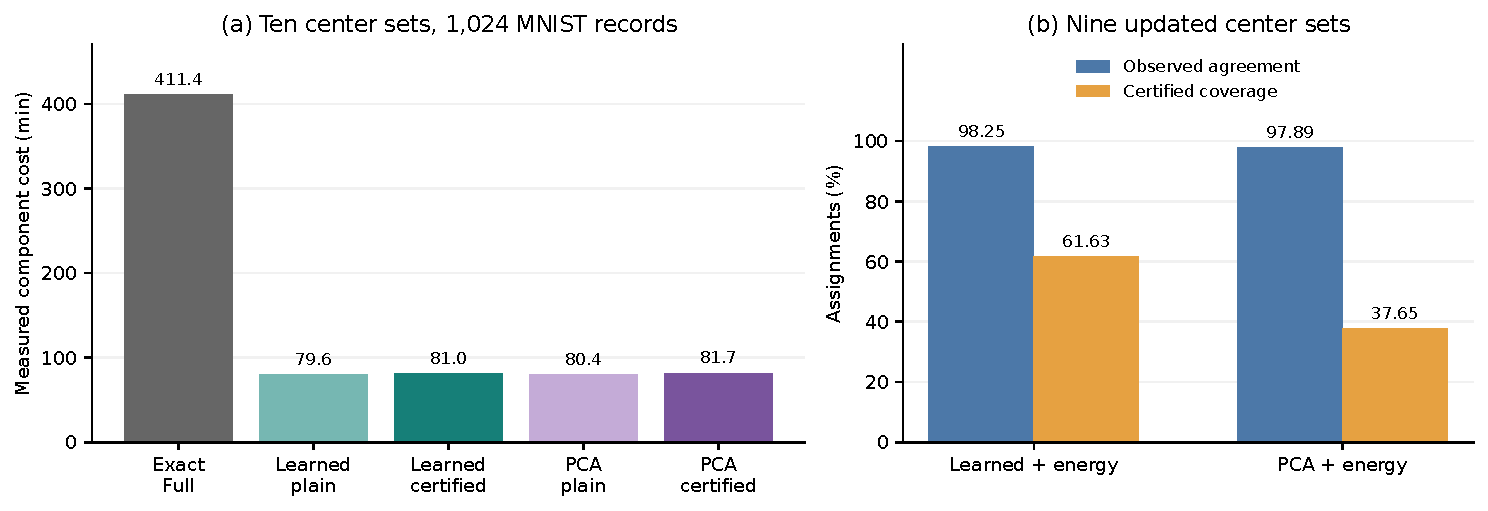
\includegraphics[width=\textwidth]{paper_results/review_controls/generated_completed_20261020/matched_scale.pdf}
\caption{Completed 1,024-record MNIST audit. (a) Measured component costs across ten public center sets, with setup and preprocessing charged once per alternative. Exact Full and approximate reuse provide different fidelity guarantees. (b) Mean agreement with quantized Full and guaranteed assignment coverage across nine updated sets. High empirical agreement does not imply that every assignment is certified.}
\label{fig:matched-scale}
\end{figure*}

\subsection{Proved accuracy envelopes and representation budgets}
The cost reductions come with a different verification contract. At $N=1024$, learned/energy agrees with quantized Full on 98.25\% of assignments on average across updated sets, while the proved correct-assignment count covers 61.63\% of rows on average and falls to 21.09\% for the worst update. Mean relative cost-interval width is 20.65\%. PCA gives 97.89\% agreement, 37.65\% coverage and 37.97\% width. Table~\ref{tab:matched-certificate-quality} reports all four main catalogs. Certified coverage is a lower bound for each individual set; an average across sets is descriptive and cannot replace its particular certificate.
\begin{table*}[tp]
\caption{Completed integer certificate quality at rank 15, $T=4096$. Agreement, certified coverage and relative cost-interval width are means across nine updated center sets. All checked intervals contain the exact quantized optimum; no certified assignment is incorrect.}\label{tab:matched-certificate-quality}
\centering\small
\begin{adjustbox}{max width=\textwidth}
\begin{tabular}{@{}llrrr@{}}
\toprule
Catalog & Method & Agreement (\%) & Certified (\%) & Width (\%) \\
\midrule
CIFAR/ResNet $N=64$ & Learned + energy & 99.48 & 60.76 & 24.00 \\
CIFAR/ResNet $N=64$ & PCA + energy & 98.44 & 39.76 & 33.58 \\
MNIST $N=1024$ & Learned + energy & 98.25 & 61.63 & 20.65 \\
MNIST $N=1024$ & PCA + energy & 97.89 & 37.65 & 37.97 \\
MNIST $N=256$ & Learned + energy & 98.31 & 59.20 & 20.51 \\
MNIST $N=256$ & PCA + energy & 97.44 & 35.98 & 38.10 \\
MNIST $N=64$ & Learned + energy & 98.26 & 52.26 & 20.80 \\
MNIST $N=64$ & PCA + energy & 96.53 & 30.03 & 38.19 \\
\bottomrule
\end{tabular}
\end{adjustbox}
\end{table*}


All 100 proved method/set outputs match the independent Python integer certificate, including assignment flags, count and both cost endpoints. Across 33,280 record/set evaluations, no certified assignment is incorrect and no interval misses the exact quantized optimum. These finite checks test implementation consistency; Proposition~\ref{prop:integer-envelope} supplies the general bound. The reported certified fractions and interval widths describe the guarantee available for each task without assigning a universal pass/fail threshold. The measured cost ratios do not establish equally exact services or authorize using small empirical point errors in place of the certificate.

The completed higher-rank proof pilots improve accuracy and certificate utility at increased component cost (Table~\ref{tab:proved-certificate-budget}). On MNIST $N=256$, learned rank-63/$T=16384$ gives 99.74\% agreement, 85.20\% certified coverage and 7.26\% mean width. Plain and certified totals are 1,731.2 and 1,834.8\,s, versus 1,274.3 and 1,309.2\,s at rank 15. PCA's higher-rank counterpart gives 99.70\% agreement, 80.51\% coverage and 8.88\% width. Both pilots replay all 576 proofs per case, including Stage~1. Rank, basis precision and query batch change together; these are combined configuration effects rather than an isolated causal effect of rank.
\begin{table*}[tp]
\caption{Completed predeclared MNIST $N=256$ rank-63, $T=16384$ proof pilots (batch 16). Quality means exclude the deployed set; costs cover all ten sets. Rank, precision and batching change together, so cost differences are configuration effects rather than an isolated rank ablation.}\label{tab:proved-certificate-budget}
\centering\small
\begin{adjustbox}{max width=\textwidth}
\begin{tabular}{@{}lllllll@{}}
\toprule
Method & Plain (s) & Certified (s) & Full / certified & Agreement (\%) & Certified (\%) & Width (\%) \\
\midrule
Learned + energy & 1,731.2 & 1,834.8 & 3.40 & 99.74 & 85.20 & 7.26 \\
PCA + energy & 1,753.5 & 1,850.1 & 3.37 & 99.70 & 80.51 & 8.88 \\
\bottomrule
\end{tabular}
\end{adjustbox}
\end{table*}


The native controls are retained separately in the artifact. The 1,024-record catalog extends the same held-out MNIST ordering; its first 256 quantized rows exactly match the earlier catalog. The deployed basis, scales, salts and ten center sets are retained without fitting on added audit rows. The original native preflight contains 80 method/set cells and 28,160 record/set evaluations; its rank-15 cases overlap the subsequently proved controls and are not independent observations.

A training-only native budget grid evaluates ranks 15/31/63/127 and basis scales 4096/16384 on the same 1,024 rows and ten sets. All cells are retained, and the rank-63 high-scale proof pilots were specified before inspecting these outcomes. Rank 15's high-scale control rescales the original rounded basis; larger ranks fit training data and round at each scale. At rank 63 and $T=16384$, learned/energy obtains 99.75\% agreement, 85.84\% mean coverage and 7.37\% width; rank 127 gives 90.32\% coverage and 4.64\% width. PCA also improves (Table~\ref{tab:native-certificate-budget}). These higher-rank 1,024-record cells are native calculations, not proof benchmarks; only the 256-record rank-63 configurations above have measured proof costs.
\begin{table*}[tp]
\caption{Native MNIST $N=1024$ budget controls (nine updated sets, quantized Full reference). All ranks and both basis scales are retained in the CSV artifact; this table shows the original configuration and larger-rank high-scale controls. These are not proof benchmarks.}\label{tab:native-certificate-budget}
\centering\small
\begin{adjustbox}{max width=\textwidth}
\begin{tabular}{@{}llrrrr@{}}
\toprule
Head rank / $T$ & Method & Agreement (\%) & Certified (\%) & Worst (\%) & Width (\%) \\
\midrule
15/4096 & Learned + energy & 98.25 & 61.63 & 21.09 & 20.65 \\
15/4096 & PCA + energy & 97.89 & 37.65 & 16.02 & 37.97 \\
31/16384 & Learned + energy & 99.36 & 76.86 & 31.05 & 12.28 \\
31/16384 & PCA + energy & 99.35 & 63.43 & 29.00 & 18.53 \\
63/16384 & Learned + energy & 99.75 & 85.84 & 45.80 & 7.37 \\
63/16384 & PCA + energy & 99.71 & 81.89 & 44.92 & 8.98 \\
127/16384 & Learned + energy & 99.86 & 90.32 & 59.86 & 4.64 \\
127/16384 & PCA + energy & 99.84 & 88.61 & 60.06 & 5.22 \\
\bottomrule
\end{tabular}
\end{adjustbox}
\end{table*}


Across the complete campaign, all 6,848 proofs pass independent public-only replay: 2,000 exact Full proofs and 4,848 Stage~1/plain/certified reuse proofs. Local analysis validates 208 captured metadata hashes, approved task coverage, matching original rows and centers, exact integer Full outputs and the independent certificate outputs. Targeted tests additionally reject altered roots, keys, indices, assignments and valid-range changes to certificate outputs. Optional tolerance-checker tests apply different user requirements to the same valid smoke certificate, separately from proof verification. The measurements themselves are reported as certified counts, cost intervals and observed agreement; application-specific tolerances are not treated as a benchmark success criterion.


\subsection{Fixed-center fidelity and the cached baseline}\label{sec:results}
On the full-cached five-start study, head+energy has mean ARI 0.999647 and agreement 99.9845\% against quantized Full, compared with PCA-16's 0.933384 and 97.2146\%. Against floating Full, head+energy agreement is 99.9108\%, while quantized Full itself reaches 99.9129\%. This separates input rounding from the additional basis-rounding effect. Table~\ref{tab:full-accuracy} gives the corpus/$k$ values; the capped eight-corpus results appear in Appendix~\ref{app:fixed}.
\begin{table*}[tp]
\caption{Native fidelity on all cached image rows and nonzero cached text-training rows.}\label{tab:full-accuracy}
\centering\small
\begin{adjustbox}{max width=\textwidth}
\begin{tabular}{@{}lrrrrrr@{}}
\toprule
Corpus & $k$ & PCA ARI$_Q$ & Ours ARI$_Q$ & PCA agree.$_Q$ (\%) & Ours agree.$_Q$ (\%) & Ours agree.$_F$ (\%) \\
\midrule
MNIST & 5 & 0.97712 & 0.99974 & 99.072 & 99.990 & 99.989 \\
MNIST & 10 & 0.93466 & 0.99975 & 96.956 & 99.989 & 99.989 \\
Fashion-MNIST & 5 & 0.99601 & 0.99987 & 99.831 & 99.994 & 99.995 \\
Fashion-MNIST & 10 & 0.98809 & 0.99988 & 99.416 & 99.994 & 99.994 \\
20 Newsgroups & 5 & 0.88163 & 0.99920 & 95.724 & 99.968 & 99.712 \\
20 Newsgroups & 10 & 0.82280 & 0.99945 & 92.289 & 99.973 & 99.785 \\
\bottomrule
\end{tabular}
\end{adjustbox}
\par\vspace{3pt}\begin{minipage}{0.98\textwidth}\footnotesize Subscripts $Q$ and $F$ denote quantized-Full and floating-Full references. Five fitted starts per corpus/$k$; 60/40 fitting/audit split. MNIST and Fashion-MNIST: 70,000 rows each (28,000 audit rows). Text: 10,944 nonzero training documents, 2,000 TF--IDF features (4,378 audit rows). These are native runs, not whole-corpus proofs. Ours denotes both head/energy variants.\end{minipage}
\end{table*}


The earlier Poseidon2 fixed-center proof cohort provides the relevant control. For one whole-catalog MNIST query with $N=64$, head+energy+JL requires 306,274 constraints and 5.09\,s of proving, PCA-16 requires 472,429 and 6.30\,s, and cached exact answers require 197,147 and 3.44\,s. Its matched no-tail head+energy control has the same answers; the optional tail is unused by the fixed-center query. Including preprocessing in four distinct 32-row subset queries gives 268.38\,s for head+energy+JL versus 279.12\,s for PCA and 246.66\,s for cached answers (Appendix~\ref{app:fixed}). Thus the single-set evidence favors the exact cached baseline, motivating the changing-center workload.

The completed five-start capped follow-up independently checks fixed-center numerical fidelity (Table~\ref{tab:fixed-five-starts}). At total width 16, the protected head with a JL residual tail has 100\% mean assignment agreement in floating arithmetic and 99.987\% after input/basis rounding, versus 95.340\% for plain PCA and 62.409\% for sparse JL. Its integer mean absolute cost error is 3.114\%, because this control estimates residual cost with a random tail. It is not the head+energy representation used by the main reuse circuit, and plain PCA here is not the stronger PCA+energy baseline. These native results support fixed-center fidelity rather than an additional proof-speed claim.
\begin{table*}[tp]
\caption{Five-start fixed-center fidelity at total width 16 on the capped eight-corpus campaign.}\label{tab:fixed-five-starts}
\centering\small
\begin{adjustbox}{max width=\textwidth}
\begin{tabular}{@{}lrrrrr@{}}
\toprule
Corpus & Head/JL float (\%) & Head/JL int. (\%) & PCA (\%) & Sparse JL (\%) & Int. $|e_\Psi|$ (\%) \\
\midrule
Gaussian-easy & 100.000 & 100.000 & 100.000 & 89.240 & 2.977 \\
Gaussian-hard & 100.000 & 100.000 & 98.600 & 45.235 & 1.297 \\
Margin synthetic & 100.000 & 99.975 & 82.950 & 60.350 & 2.833 \\
MNIST & 100.000 & 99.990 & 97.850 & 66.036 & 4.431 \\
Fashion-MNIST & 100.000 & 100.000 & 99.600 & 82.540 & 3.610 \\
Gisette & 100.000 & 99.967 & 97.767 & 45.371 & 1.718 \\
Arcene & 100.000 & 100.000 & 99.000 & 86.775 & 7.116 \\
20 Newsgroups & 100.000 & 99.966 & 86.955 & 23.726 & 0.927 \\
Mean & 100.000 & 99.987 & 95.340 & 62.409 & 3.114 \\
\bottomrule
\end{tabular}
\end{adjustbox}
\par\smallskip\begin{minipage}{0.98\textwidth}\footnotesize Assignment agreement is against floating original-space Full. There are 80 corpus/$k$/start cells (eight corpora, $k=5,10$, five starts); ten random maps are averaged within each cell. Head/JL preserves the deployed-center head and uses a sparse residual tail, not the energy statistic of the main reuse method. PCA here is plain PCA, not PCA with energy. The final column is mean absolute cost error of the integer Head/JL method. These native runs do not measure proof performance.\end{minipage}
\end{table*}


\subsection{Historical changing-center reuse: cumulative proof cost}
The workload audits the same catalog against ten center sets in this fixed order: the deployed set, two independent refits, two half-training subsample refits, Lloyd iterates 1/3/10 from another initialization, and perturbations of size 0.1/0.3 of median deployed-center spacing. These scenarios retain $k=5$. They use training data and do not form an optimization loop driven by private audit outputs. All methods receive the same integer catalog and quantized center sets.

Table~\ref{tab:reuse-cost} and Fig.~\ref{fig:reuse-cost} show the historical amortization comparison. For MNIST $N=64$, learned head+energy costs 311.4\,s at one set, 317.7\,s at two and 368.8\,s at ten. The center-specific cached baseline costs 250.1, 502.2 and 2,540.9\,s, respectively. For CIFAR embeddings, the ten-set totals are 635.2\,s versus 4,928.8\,s. The $N=256$ MNIST check gives 941.2, 977.4 and 1,267.6\,s for learned head+energy, versus 860.9, 1,724.8 and 8,642.8\,s for cached. The learned method crosses cached at $L=2$ in all three workloads; ten-set ratios are 6.89, 7.76 and 6.82. PCA+energy has essentially the same reuse cost: 366.2, 635.6 and 1,265.0\,s at ten sets. The result is amortization across changing centers, not faster individual query proofs than cached answers.
\begin{table*}[tp]
\caption{Cumulative cost across successive center sets, query batch $b=64$, $k=5$ (seconds).}\label{tab:reuse-cost}
\centering\small
\begin{adjustbox}{max width=\textwidth}
\begin{tabular}{@{}llrrr@{}}
\toprule
Catalog & Method & $L=1$ & $L=2$ & $L=10$ \\
\midrule
MNIST ($N=64$) & Cached exact & 250.1 & 502.2 & 2,540.9 \\
MNIST ($N=64$) & Exact affine & 277.9 & 552.0 & 2,758.4 \\
MNIST ($N=64$) & Full (extrapolated) & 342.3 & 684.6 & 3,473.6 \\
MNIST ($N=64$) & Span + energy & 282.3 & 287.4 & 329.1 \\
MNIST ($N=64$) & PCA + energy & 309.5 & 315.9 & 366.2 \\
MNIST ($N=64$) & Learned head + energy & 311.4 & 317.7 & 368.8 \\
CIFAR/ResNet-50 ($N=64$) & Cached exact & 490.3 & 980.3 & 4,928.8 \\
CIFAR/ResNet-50 ($N=64$) & Exact affine & 517.4 & 1,029.7 & 5,099.5 \\
CIFAR/ResNet-50 ($N=64$) & Full (extrapolated) & 493.6 & 984.2 & 4,781.0 \\
CIFAR/ResNet-50 ($N=64$) & Span + energy & 515.6 & 520.9 & 563.2 \\
CIFAR/ResNet-50 ($N=64$) & PCA + energy & 555.3 & 563.7 & 635.6 \\
CIFAR/ResNet-50 ($N=64$) & Learned head + energy & 554.9 & 563.7 & 635.2 \\
MNIST ($N=256$) & Cached exact & 860.9 & 1,724.8 & 8,642.8 \\
MNIST ($N=256$) & Exact affine & 889.4 & 1,777.1 & 8,851.4 \\
MNIST ($N=256$) & Full (extrapolated) & 808.9 & 1,574.4 & 8,036.5 \\
MNIST ($N=256$) & Span + energy & 904.2 & 926.4 & 1,105.6 \\
MNIST ($N=256$) & PCA + energy & 940.5 & 977.1 & 1,265.0 \\
MNIST ($N=256$) & Learned head + energy & 941.2 & 977.4 & 1,267.6 \\
\bottomrule
\end{tabular}
\end{adjustbox}
\par\smallskip\begin{minipage}{0.98\textwidth}\footnotesize Totals add measured native preparation, compilation, setup, witness generation and median proving times. All compressed/cached/affine catalog proofs were generated; Full catalog proving is extrapolated from one measured batch per set. The deployed set is first. Verification, fitting, warmups, I/O and public new-center preparation are excluded.\end{minipage}
\end{table*}

\begin{figure*}[tp]
\centering
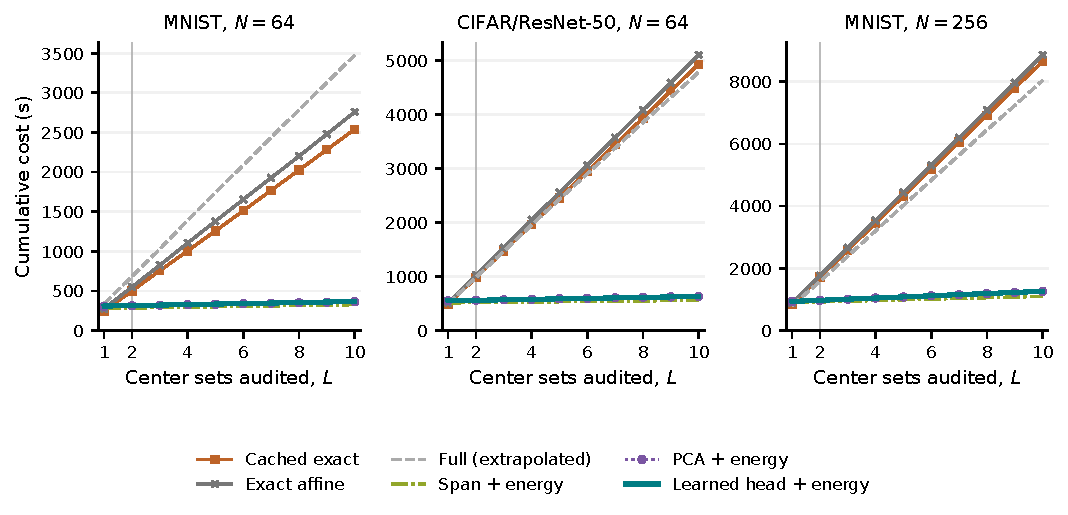
\includegraphics[width=\textwidth]{paper_results/reuse_revision/generated_20261020/cumulative_cost.pdf}
\caption{Historical cumulative cost for three completed changing-center workloads. The comparator Full embeds centers; this figure does not evaluate public-center Full. Learned head and PCA with energy almost overlap; savings over the tested center-specific cached/affine baselines come from reusing preprocessing and setup. The vertical line marks the second center set. Full catalog proving is extrapolated from one measured batch per set.}
\label{fig:reuse-cost}
\end{figure*}

For MNIST $N=64$, learned and PCA with energy have the same 519,896-constraint reuse circuit, compared with 343,455 for the narrower span-only head. Their Stage~1 circuits have 171,586 and 171,582 constraints per row. At $N=256$, the larger Merkle depth increases the shared reuse circuit to 568,022 constraints; learned Stage~1 uses 173,086 per row. For CIFAR, learned/PCA reuse requires 524,336 constraints and Stage~1 requires 432,049 per row. Selecting a different basis can therefore change accuracy without materially changing proof cost. Saved peak process-tree RSS is about 1.1--1.6\,GB for the 16-statistic methods; it excludes the Python driver and is not whole-pipeline memory.

\subsection{Changing-center fidelity}
The learned head has higher new-center agreement than PCA with energy on all three proof workloads: 98.26\% versus 96.53\% on MNIST $N=64$, 99.48\% versus 98.44\% on CIFAR embeddings, and 98.31\% versus 97.44\% on MNIST $N=256$ (Table~\ref{tab:reuse-quality}). The narrower deployed span alone reaches 83.51\%, 96.35\% and 85.76\%. Learned mean absolute cost errors are 0.228\%, 0.338\% and 0.178\%, compared with PCA/energy's 1.536\%, 0.441\% and 1.722\%. Cached and affine attain 100\% agreement, with small floating-reference cost differences due to quantization. Mean agreement is not a worst-case guarantee: learned agreement on the least accurate updated set is 95.31\%, 96.88\% and 94.92\%, respectively.
\begin{table*}[tp]
\caption{Answer fidelity on the nine new center sets in each proof workload.}\label{tab:reuse-quality}
\centering\small
\begin{adjustbox}{max width=\textwidth}
\begin{tabular}{@{}llrrr@{}}
\toprule
Catalog & Method & Mean agree. (\%) & Min. agree. (\%) & Mean $|e_\Psi|$ (\%) \\
\midrule
MNIST ($N=64$) & Cached exact & 100.00 & 100.00 & 0.003 \\
MNIST ($N=64$) & Exact affine & 100.00 & 100.00 & 0.003 \\
MNIST ($N=64$) & Span + energy & 83.51 & 67.19 & 1.977 \\
MNIST ($N=64$) & PCA + energy & 96.53 & 93.75 & 1.536 \\
MNIST ($N=64$) & Learned head + energy & 98.26 & 95.31 & 0.228 \\
CIFAR/ResNet-50 ($N=64$) & Cached exact & 100.00 & 100.00 & 0.002 \\
CIFAR/ResNet-50 ($N=64$) & Exact affine & 100.00 & 100.00 & 0.002 \\
CIFAR/ResNet-50 ($N=64$) & Span + energy & 96.35 & 89.06 & 0.757 \\
CIFAR/ResNet-50 ($N=64$) & PCA + energy & 98.44 & 96.88 & 0.441 \\
CIFAR/ResNet-50 ($N=64$) & Learned head + energy & 99.48 & 96.88 & 0.338 \\
MNIST ($N=256$) & Cached exact & 100.00 & 100.00 & 0.004 \\
MNIST ($N=256$) & Exact affine & 100.00 & 100.00 & 0.004 \\
MNIST ($N=256$) & Span + energy & 85.76 & 64.84 & 2.219 \\
MNIST ($N=256$) & PCA + energy & 97.44 & 95.31 & 1.722 \\
MNIST ($N=256$) & Learned head + energy & 98.31 & 94.92 & 0.178 \\
\bottomrule
\end{tabular}
\end{adjustbox}
\par\smallskip\begin{minipage}{0.98\textwidth}\footnotesize Agreement is against floating-point original-space Full on the same catalog rows. Means weight the nine new center sets equally; minimum is the worst set, not a confidence bound. Cached and affine are exact on quantized inputs, so their floating-reference cost errors can be nonzero.\end{minipage}
\end{table*}

This is an accuracy--reuse trade-off against exact recomputation and an accuracy comparison at similar proof cost against PCA. The nine updated sets reuse the same rows and fitted basis, so they are not nine independent dataset replications.

\subsection{Native new-center, shift and owner controls}
The broader native new-center grid evaluates budgets 16/32/64/128/256, two sparse-map densities and ten maps per randomized setting, subject to input dimension and PCA training-rank restrictions. It includes twelve new scenarios, adding changed center counts and another Lloyd snapshot to the proof workload's families. On matched cells, head+energy with a JL residual cross-term estimate is less accurate than PCA+energy at every tested budget. At budget 16 the agreement is 73.92\% versus 93.27\%; at 256 it is 91.16\% versus 98.13\% (Table~\ref{tab:reuse-jl}). The real same-center control gives 100\% agreement and maximum absolute relative cost error below $1.5\times10^{-15}$.
\begin{table*}[tp]
\caption{Native new-center comparison on matched cells: head/energy/JL versus PCA/energy.}\label{tab:reuse-jl}
\centering\small
\begin{adjustbox}{max width=\textwidth}
\begin{tabular}{@{}rrrrrr@{}}
\toprule
Budget & Cells & JL agree. (\%) & PCA/E agree. (\%) & JL $|e_\Psi|$ (\%) & PCA/E $|e_\Psi|$ (\%) \\
\midrule
16 & 720 & 73.92 & 93.27 & 5.852 & 0.673 \\
64 & 648 & 85.34 & 96.14 & 1.110 & 0.152 \\
256 & 504 & 91.16 & 98.13 & 0.326 & 0.037 \\
\bottomrule
\end{tabular}
\end{adjustbox}
\par\smallskip\begin{minipage}{0.98\textwidth}\footnotesize The tail estimates the residual cross term with one signed bucket per column. Maps are averaged within a corpus/$k$/start/scenario cell before aggregation. Eligibility differs across budgets; within each row both methods use identical cells. Native float64 computation, not proofs.\end{minipage}
\end{table*}


A follow-up tests learned-head/JL budget splits, $q=4,8$, SRHT maps, clipping and shrinkage. No tested hybrid improves the mean agreement over PCA with energy on its matched cells at any tested budget. The full learned head without a tail is also slightly below PCA/energy in this broader native comparison: 93.19\% versus 93.27\% agreement at budget 16, and 98.07\% versus 98.13\% at 256. Thus the learned method's higher agreement on the two proof catalogs does not extend to the aggregate native grid. The results motivate spending the residual budget on learned directions instead of a random cross-term estimator for the main circuit, while retaining PCA/energy as a strong baseline.

The shift/owner study comprises 60 jobs and 22,260 rows across five corpora. The owner simulation partitions training records among five owners with Dirichlet parameter 0.3; the residual/PCA basis sees only owner~0, while deployed public centers come from pooled training data. The shift simulation fits on old classes and tests new-only and mixed-class cases. At budget 16, learned head+energy reaches 89.89\% agreement versus 81.71\% for PCA/energy in the owner setting, but 74.50\% versus 76.33\% under shift. JL is weaker in both aggregate comparisons (Table~\ref{tab:reuse-shift}). These are native simulations with different information constraints, not federated proof or communication measurements.
\begin{table*}[tp]
\caption{Native budget-16 agreement under non-IID owners and class distribution shift.}\label{tab:reuse-shift}
\centering\small
\begin{adjustbox}{max width=\textwidth}
\begin{tabular}{@{}llrrr@{}}
\toprule
Setting & Method & Cells & Agree. (\%) & Matched PCA/E (\%) \\
\midrule
owners & Learned head + energy & 360 & 89.89 & 81.71 \\
shift & Learned head + energy & 60 & 74.50 & 76.33 \\
owners & Head/energy/JL ($q=4$) & 360 & 72.02 & 81.71 \\
shift & Head/energy/JL ($q=4$) & 60 & 60.14 & 76.33 \\
owners & Plain JL ($q=4$) & 360 & 55.38 & 81.71 \\
shift & Plain JL ($q=4$) & 60 & 58.48 & 76.33 \\
\bottomrule
\end{tabular}
\end{adjustbox}
\par\smallskip\begin{minipage}{0.98\textwidth}\footnotesize Five corpora, $k=5,10$, three starts. Random maps are averaged within each matched cell. Owners: residual/PCA fitting uses owner 0, while deployed public centers use pooled training rows. Shift: fit on old classes and audit new-only/mixed cases. These are native simulations.\end{minipage}
\end{table*}


\subsection{Binding and adaptive-map controls}
The existing circuit tests exercise honest in-span and out-of-span reuse, check that the in-span integer fixture agrees with Full, and reject altered costs, margins, assignments, authenticated heads and offsets. Earlier original-binding tests also cover missing Stage~1 indices, substituted roots and keys, and changed subset data. These are targeted engineering checks of the implemented relation.

The earlier native adaptive-map controls illustrate a different question (Table~\ref{tab:attack-controls}). With a known PCA map, the constructed perturbation changes about 97.6\% of assignments while leaving the projected claim unchanged. The corresponding fresh sparse-map control does not hide the same injected energy. These controls generate no forged end-to-end proofs and test a linear head/tail representation, not head+energy. They show why a faithfully executed known projection can be a poor proxy on adversarial data; the Stage~1 binding guarantee itself does not depend on a JL tail.
The detailed native perturbation table is retained in Appendix~\ref{app:attack}.

\section{Discussion}\label{sec:discussion}
\subsection{Choosing the representation}
For a single approved center set with repeated subset queries, cached exact answers are the strongest tested choice: the original-space integer argmin and cost are proved once and later authenticated cheaply. Affine scores retain all candidate fixed-center distances and are exact on the same integer inputs. Head and energy are useful when a common represented span supports several center sets, or when later approximate audits justify retaining more information than one cached answer.

The learned representation targets the latter use. Protecting the deployed span preserves its real-arithmetic comparisons, while residual PCA spends the remaining budget on training directions likely to matter for updates. The main proof workloads show a favorable combination of reuse cost and agreement, rather than a proof-speed advantage over equally reusable PCA with energy. The distribution-shift study further shows that learned head is not uniformly more accurate than PCA. Basis selection is an approximation policy that should be approved and evaluated for the intended queries.

The tested sparse-JL tails have a distinct reason to remain in the study: choosing a map without training data and analyzing its dependence on commitment order. Their negative fidelity results are evidence about the tested estimators and budgets. They neither invalidate JL theory nor establish that learned maps have a worst-case accuracy guarantee. Stage~1 binding applies to either approved map.

\subsection{Scope and limitations}
The completed review-control evidence covers actual MNIST catalogs of 64, 256 and 1,024 records and a 64-record CIFAR/ResNet catalog, each with ten ordered center sets on one four-CPU Linux host. It also includes two 256-record higher-rank proof configurations. The larger MNIST catalogs are scale checks on the same corpus and fitted-model configuration, not independent applications. New-center sets are refits, subsamples, Lloyd snapshots and perturbations from a fixed training corpus. The completed eight-corpus five-start native campaign broadens fixed-center fidelity evidence, but does not substitute for independent-model or cross-host proof replication. A 1,024-record proof catalog remains much smaller than a production-scale embedding collection.

Cumulative costs reconstruct measured components; they are not observed online deployment latency. They exclude public-model fitting, verification, warmups, I/O and new-center-statistic preparation. Historical Full totals extrapolate catalog proving and charge center-specific setup. The completed exact public-center Full controls remove both limitations: one setup serves all ten sets and every catalog batch is proved. The new export consistently includes native answer construction. At $N=1024$, component-cost ratios are 5.17 for plain learned reuse and 5.08 for certified reuse. These are resource-bounded configurations with different feasible batch sizes and one measured repetition per sample; they do not establish an optimal exact implementation or a cross-host performance distribution. An in-span reusable affine parameterization remains another possible exact design for restricted center updates.

Plain reuse proves approximate original-space scores with exact execution of the approved integer relation. The optional certificate adds a conservative bound for each approved center set, but does not turn every approximate assignment into an exact one. Certified coverage can be much lower than observed agreement, and none of the updated proved cases meets the illustrative strict 99\%/1\% policy. Such an auditor should request exact Full. At rank 15, certificate overhead on learned total component cost falls from 14.26\% at $N=64$ to 1.74\% at $N=1024$, where shared preprocessing dominates. The proved rank-63 configuration improves coverage but changes precision and batching too. Selective exact refinement of uncertified rows is a future implementation option, not a completed result.

The standalone public-only verifier is now implemented and exercised on smoke bundles, and it is required for every new completed campaign case. Historical in-process verification counts still do not imply fresh replay of every old saved bundle. The study excludes proof of model training, real federated communication, adaptive leakage bounds, cross-host replication and full-corpus proof deployment. A real model-update trace would further test deployment relevance.

\subsection{Contribution and submission boundary}
The projection identity, residual norm inequalities, matrix row-sum bound and Groth16 backend are established ingredients. The contribution is their explicit composition into an original-data-bound reusable audit with checked integer error envelopes, independently approved public tasks and a quality acceptance policy. The completed proof controls and native budget grid measure certified utility rather than only empirical fidelity, while public-center Full prevents attributing setup amortization to compression alone. This is a systems contribution relevant to repeated verification of clustering and prototype updates. Its application value depends on the auditor's permitted error; the strict policy failures remain part of the result. It supplies neither a new general dimensionality-reduction theorem nor universal learned-over-PCA improvement. Author metadata, declarations and scientific approval remain necessary before submission.

\section{Conclusion}\label{sec:conclusion}
Classical head coordinates and residual energy provide a compact interface for verifiable center-based audits. The system binds their integer derivation to committed original rows and reuses the catalog across public center updates. Optional certificates prove a lower bound on correct quantized original-space assignments and a cost interval, allowing an auditor to refuse an approximate answer under an explicit tolerance. The completed 14-case campaign includes actual 1,024-record proofs and 6,848 independent public-only verifications. At that scale, learned certified reuse has 5.08-fold lower measured component cost than exact public-center Full, with 98.25\% observed assignment agreement but only 61.63\% mean certified coverage. The higher-rank proof pilots improve certified utility at increased total cost, while every updated case still fails the strict illustrative policy. The result is a measured computation--accuracy trade-off for reusable audits, rather than equal-fidelity acceleration of exact clustering or uniform superiority over PCA.


\FloatBarrier
\onecolumn
\appendix
\numberwithin{table}{section}
\renewcommand{\thetable}{\Alph{section}.\arabic{table}}
\renewcommand{\theHtable}{appendix.\Alph{section}.\arabic{table}}
\renewcommand{\theHequation}{appendix.\Alph{section}.\arabic{equation}}
\section{Additional fixed-center evidence}\label{app:fixed}
The tables in this appendix retain the earlier completed Poseidon2 cohort and its native component/five-start follow-ups. They are not pooled with the new changing-center timing cohort. ``CommitJL'' in these retained tables means the protected head, energy and optional sparse tail; fixed-center assignment/cost queries do not use the tail. Native accuracy compares with quantized Full unless marked otherwise.
% Numerical contents retained from bound_revision; regular floats for the single-column appendix.
\begin{table}[!htbp]
\caption{Fixed-center fidelity on eight capped corpora at storage budget 16.}\label{tab:capped}
\centering\small
\begin{adjustbox}{max width=\textwidth}
\begin{tabular}{@{}lrrrrrr@{}}
\toprule
Corpus & $k$ & Sparse ARI & PCA ARI & Head/E ARI & PCA agree. (\%) & Head/E agree. (\%) \\
\midrule
Gaussian-easy & 5 & 0.62947 & 1.00000 & 1.00000 & 100.000 & 100.000 \\
Gaussian-easy & 10 & 0.87790 & 1.00000 & 1.00000 & 100.000 & 100.000 \\
Gaussian-hard & 5 & 0.11602 & 0.99365 & 1.00000 & 99.792 & 100.000 \\
Gaussian-hard & 10 & 0.15151 & 0.99359 & 1.00000 & 99.000 & 100.000 \\
Margin-synthetic & 5 & 0.18329 & 0.62386 & 0.99640 & 89.833 & 99.917 \\
Margin-synthetic & 10 & 0.21543 & 0.49844 & 1.00000 & 79.167 & 100.000 \\
MNIST & 5 & 0.36872 & 0.98165 & 0.99960 & 99.183 & 99.983 \\
MNIST & 10 & 0.36090 & 0.92547 & 0.99964 & 96.567 & 99.983 \\
Fashion-MNIST & 5 & 0.66488 & 0.99484 & 1.00000 & 99.783 & 100.000 \\
Fashion-MNIST & 10 & 0.64867 & 0.98679 & 0.99958 & 99.317 & 99.983 \\
Gisette & 5 & 0.14792 & 0.96671 & 0.99917 & 98.694 & 99.972 \\
Gisette & 10 & 0.12200 & 0.92786 & 1.00000 & 96.861 & 100.000 \\
Arcene & 5 & 0.85164 & 1.00000 & 1.00000 & 100.000 & 100.000 \\
Arcene & 10 & 0.67673 & 0.95751 & 1.00000 & 97.500 & 100.000 \\
20 Newsgroups & 5 & 0.01789 & 0.82891 & 1.00000 & 93.511 & 100.000 \\
20 Newsgroups & 10 & 0.00868 & 0.61244 & 1.00000 & 78.988 & 100.000 \\
\bottomrule
\end{tabular}
\end{adjustbox}
\par\vspace{3pt}\begin{minipage}{0.98\textwidth}\footnotesize Reference: quantized Full. Means over three fitted starts; sparse maps are averaged within a start before aggregation. Head/E and CommitJL have identical fixed-center outputs. Sparse JL uses one signed bucket per input column. ARI measures assignment fidelity, not agreement with class labels.\end{minipage}
\end{table}

\begin{table}[!htbp]
\caption{Actual whole-catalog query on 64 committed MNIST records, $k=5$.}\label{tab:query64}
\centering\small
\begin{adjustbox}{max width=\textwidth}
\begin{tabular}{@{}lrr@{}}
\toprule
Method & Constraints & Proving time (s) \\
\midrule
PCA-16 & 472,429 & 6.303 \\
Head + energy & 306,275 & 5.341 \\
CommitJL-16 & 306,274 & 5.087 \\
Exact affine & 271,205 & 5.240 \\
Cached exact & 197,147 & 3.442 \\
\bottomrule
\end{tabular}
\end{adjustbox}
\par\vspace{3pt}\begin{minipage}{0.98\textwidth}\footnotesize Same original catalog and centers for all methods; each saved proof independently verifies. This is one possible 64-record subset, with three timing repetitions after warmup. Full was measured only at $q=1$ for this catalog; no large-shape Full estimate is inserted. The one-constraint head/E difference comes from compiled context details, not useful tail computation.\end{minipage}
\end{table}

\begin{table}[!htbp]
\caption{Preprocessing and reconstructed fresh-workload cost, MNIST $N=64$, $k=5$.}\label{tab:preprocessing}
\centering\small
\begin{adjustbox}{max width=\textwidth}
\begin{tabular}{@{}lrrrrr@{}}
\toprule
Method & \shortstack{Stage-1\\constraints/row} & \shortstack{Median row\\proof (s)} & \shortstack{All row\\proofs (s)} & \shortstack{Stage-1\\compile/setup (s)} & \shortstack{Four-query\\workload (s)} \\
\midrule
PCA-16 & 170,744 & 3.087 & 197.961 & 29.011 & 279.123 \\
Head + energy & 168,901 & 3.067 & 196.990 & 28.372 & 264.617 \\
CommitJL-16 & 174,208 & 3.083 & 198.221 & 29.350 & 268.383 \\
Exact affine & 168,815 & 3.058 & 195.780 & 29.559 & 268.288 \\
Cached exact & 168,446 & 3.014 & 194.488 & 27.153 & 246.660 \\
\bottomrule
\end{tabular}
\end{adjustbox}
\par\vspace{3pt}\begin{minipage}{0.98\textwidth}\footnotesize The workload uses four genuinely distinct 32-record subsets. It adds native Go preparation, all 64 Stage-1 witness/proof costs, Stage-1 and query compilation/setup, and one witness/proof per subset. Public-model fitting, verification, warmups and I/O are excluded. These sums reconstruct measured components; they are not observed elapsed times or an empirical break-even threshold.\end{minipage}
\end{table}


\FloatBarrier

\Needspace{10\baselineskip}
\section{Native perturbation control}\label{app:attack}
This earlier control tests whether a native linear head/tail projection can conceal injected energy when its map is known. It does not construct a forged proof and does not attack the head+energy relation. The output definitions and limitations are retained with the original numerical values.
\begin{table}[!htbp]
\caption{Earlier native perturbation controls; no forged end-to-end proofs are generated.}\label{tab:attack-controls}
\centering\scriptsize
\begin{adjustbox}{max width=\textwidth}
\begin{tabular}{@{}lllll@{}}
\toprule
Projection/order & True inflation & Claim inflation & Flip fraction & Honest error \\
\midrule
pca\_public & 11.000 & 1.000 & 0.9762 & 0.0273 \\
protected\_commit & 11.000 & 11.010 & 0.0000 & 0.0000 \\
protected\_prepublished & 11.000 & 1.000 & 0.0000 & 0.0000 \\
sparse\_commit & 10.988 & 11.138 & 0.6082 & 0.3715 \\
sparse\_prepublished & 10.988 & 1.000 & 0.8578 & 0.3713 \\
\bottomrule
\end{tabular}
\end{adjustbox}
\par\smallskip
\begin{minipage}{\textwidth}\scriptsize Protected rows test the linear head+tail representation, not head+energy. Fresh-map rows use one independently guessed-map strategy. Flip and honest-error fractions concern different point sets and cannot be subtracted to isolate attack advantage. The unverified internal Pisot surrogate is excluded from comparisons with published methods.\end{minipage}
\end{table}

\FloatBarrier

\section{Data-oblivious sparse-map specification}\label{app:jl}
The canonical generator uses domain-separated SHAKE-256 streams for bucket indices and signs. For each original coordinate it draws $q$ distinct bucket indices by rejection and independent signs, retaining a canonical ordered encoding. Reducing a fixed-width word modulo $m$ without rejecting the biased prefix is not uniform; \path{code/commitjl/sparse_gen.py} implements the canonical rejection specification. Generator expansion and challenge approval are verifier-side checks, rather than an in-circuit XOF proof in the measured reuse system.

Under ideal independent zero-mean signs and the specified column sampling, $\mathbb E[\|Av\|^2/q]=\|v\|^2$: expand the square, cancel cross terms by sign independence, and count the $q$ diagonal contributions per coordinate. This is a first-moment statement, not a concentration bound. A tail estimator for the missing inner product uses $\langle Ar(x),Ar(c')\rangle/q$ in Eq.~\eqref{eq:new-center-exact}; its noise explains why adding a tail need not improve assignment fidelity at a fixed storage budget.

For commitment order, eligible roots and a digest of the relevant centers/task are registered before a fresh challenge. A verifier nonce, a beacon round with a registration deadline, or a commit--reveal protocol can supply the entropy. A task log must bound eligible attempts when claiming a task-level geometric failure probability. Root-derived deterministic randomness alone permits offline search over commitment salts. Public reproducibility is not sufficient to establish independence from adversarially chosen inputs.

\section{Quantization and evidence provenance}\label{app:configurations}
With per-coordinate rounding error at most $1/(2S)$, each point has Euclidean error at most $\sqrt d/(2S)$. For two points $u,v$, write the difference error as $\eta$, where $\|\eta\|\le\sqrt d/S$. Expanding $\|(u-v)+\eta\|^2$ gives the additive bound
\begin{equation}
\begin{aligned}
&\left|\|\widetilde u/S-\widetilde v/S\|^2-\|u-v\|^2\right|\\
&\qquad\le2\|u-v\|\sqrt d/S+d/S^2.
\end{aligned}
\end{equation}
Rounded-basis error and the omitted new-center cross term are separate from this input perturbation. The integer row bounds in Eq.~\eqref{eq:row-bounds} do not assert an original-space approximation ratio.

The historical export manifest is \path{paper_results/reuse_revision/generated_20261020/manifest.json}. It records input hashes, exact cumulative costs, cache crossovers and five-start coverage. The snapshot captured at 20:32 UTC on 19 October 2026 contains both $N=64$ workloads, the completed $N=256$ workload and all three native fidelity workers. Analysis checks 1,092 captured hashes, reconstructs saved proof costs, and validates all 80 corpus/$k$/start cells. Repeated legacy head-only ablations are excluded from the width-16 comparison. Earlier fixed-center manifests remain under \path{paper_results/bound_revision}. Raw arrays and proving artifacts remain in their preserved experiment folders; the paper source package contains numerical exports and provenance.

Review-control manifests under \path{paper_results/review_controls/} retain the complete native grids, predeclared pilots and read-only proof captures. The completed export validates 208 captured metadata hashes, reconstructs all four exact controls and ten plain/certified reuse cases from raw phases, checks Full integer labels/costs, and matches every certificate output to Python. All 6,848 proofs pass public-only worker replay; the local analysis additionally checks 33,280 record/set certificate evaluations. Native answer construction is normalized without changing original results. Individual labels and certificate flags are excluded from public proof exports; captured benchmark diagnostics are separate from those privacy-preserving exports. The current standalone verifier additionally rejects approved batch sizes lacking a pinned query key; the frozen campaign tasks use homogeneous batches whose complete coverage is checked separately.

\FloatBarrier
\twocolumn
\section*{Declarations}
\paragraph{Author information, contributions and acknowledgements}
Names, affiliations, corresponding-author details, contributor roles and acknowledgements require author confirmation before submission.
\paragraph{Funding and competing interests}
Funding sources and the competing-interest declaration require confirmation by all authors.
\paragraph{Data and code availability}
The experiments use the public benchmark sources cited in Table~\ref{tab:datasets-a} and synthetic data. Code, completed review-control captures, numerical exports and provenance manifests are provided at \url{https://github.com/Knowledge4Software/Zero-Knowledge-Clustering}. The portable paper source package includes the numerical exports and their provenance. Large dataset caches, raw historical runs and proving artifacts are retained separately; the repository guide states which evidence is included. Final archival identifiers and release metadata require author approval before submission.
\paragraph{Ethics and consent}
The final ethics and consent declarations require author review of the benchmark data sources and intended release. No claim of new collection of sensitive participant records is made in this study.
\paragraph{Declaration of generative AI and AI-assisted technologies in the manuscript preparation process}
OpenAI Codex assisted with source-code development, result aggregation, literature navigation, manuscript organization and language revision. Numerical claims are derived from retained experiment outputs and deterministic analysis scripts. The human authors are responsible for checking the code, sources, interpretation and complete manuscript, and for approving the final submission. AI tools are not authors.

\bibliographystyle{elsarticle-num}
\bibliography{references}
\end{document}
